% !TeX encoding = UTF-8
% !TeX spellcheck = es_ES
\documentclass{article}

\usepackage[utf8]{inputenc}
\usepackage[spanish]{babel}

\topmargin = -1.5cm
%\textwidth  = 18.5cm
\textwidth  = 18.1cm
\textheight  = 22cm
%\oddsidemargin =-1cm
\oddsidemargin =-0.7cm
%\pagestyle{empty}

\usepackage{ragged2e}
\usepackage{footmisc}

\usepackage{listings}

\usepackage{xcolor}

\definecolor{uprgreen}{RGB}{18,104,47}
\definecolor{uprgreen2}{RGB}{51,144,55}

\usepackage{hyperref}
\hypersetup{
	colorlinks=true,
	urlcolor=uprgreen2,
	linkcolor=uprgreen2
}
%\usepackage[breaklinks,colorlinks=true,linkcolor=red,citecolor=red, urlcolor=blue]{hyperref}

\usepackage{amsmath,amssymb,amsfonts,latexsym, graphicx}

\newcommand{\foot}{\fontsize{10}{13}\selectfont}
\newcommand{\notfoot}{\justifying\fontsize{13}{18}\selectfont}
\newtheorem{definition}{Definici\'on}

\begin{document}

{{\huge\color{uprgreen} Conferencia $\#$5}\hfill{\color{uprgreen} Asignatura tal}}\\
{\color{uprgreen} Lic. Alguien Alguien Alguien.\hfill \href{mailto:alguien.alguien@upr.edu.cu}{alguien.alguien@upr.edu.cu}}
{\color{uprgreen} \hrule}
\text{\ \ }
\\
\begin{center}
	\Large\color{uprgreen} Integración Numérica, Aplicaciones y Ejemplos
\end{center}
{\Large\bf\color{uprgreen} Sumario:}
\begin{itemize}
	\item[\color{uprgreen}*] Idea Geométrica de la Integral.
	\item[\color{uprgreen}*] Principales Definiciones.
	\item[\color{uprgreen}*] Propiedades de las Integrales.
	\item[\color{uprgreen}*] Integrales Inmediatas.
\end{itemize}
\begin{center}
	{\color{uprgreen}--------------------------------------------------------------------------------------------------------------------------------------------}
\end{center}

Desde la antigüedad se ha tratado de resolver los problemas de cálculo de área, debido a su gran uso práctico. Entre los problemas de cálculos de áreas más famosos tenemos el área del círculo, y uno de los primeros métodos para su resolución es conocido como la cuadratura del círculo. Esto consistía en inscribir un polígono regular de $2^n$ lados en un círculo, de la siguiente manera.

\begin{figure}[h!]
	\centering
	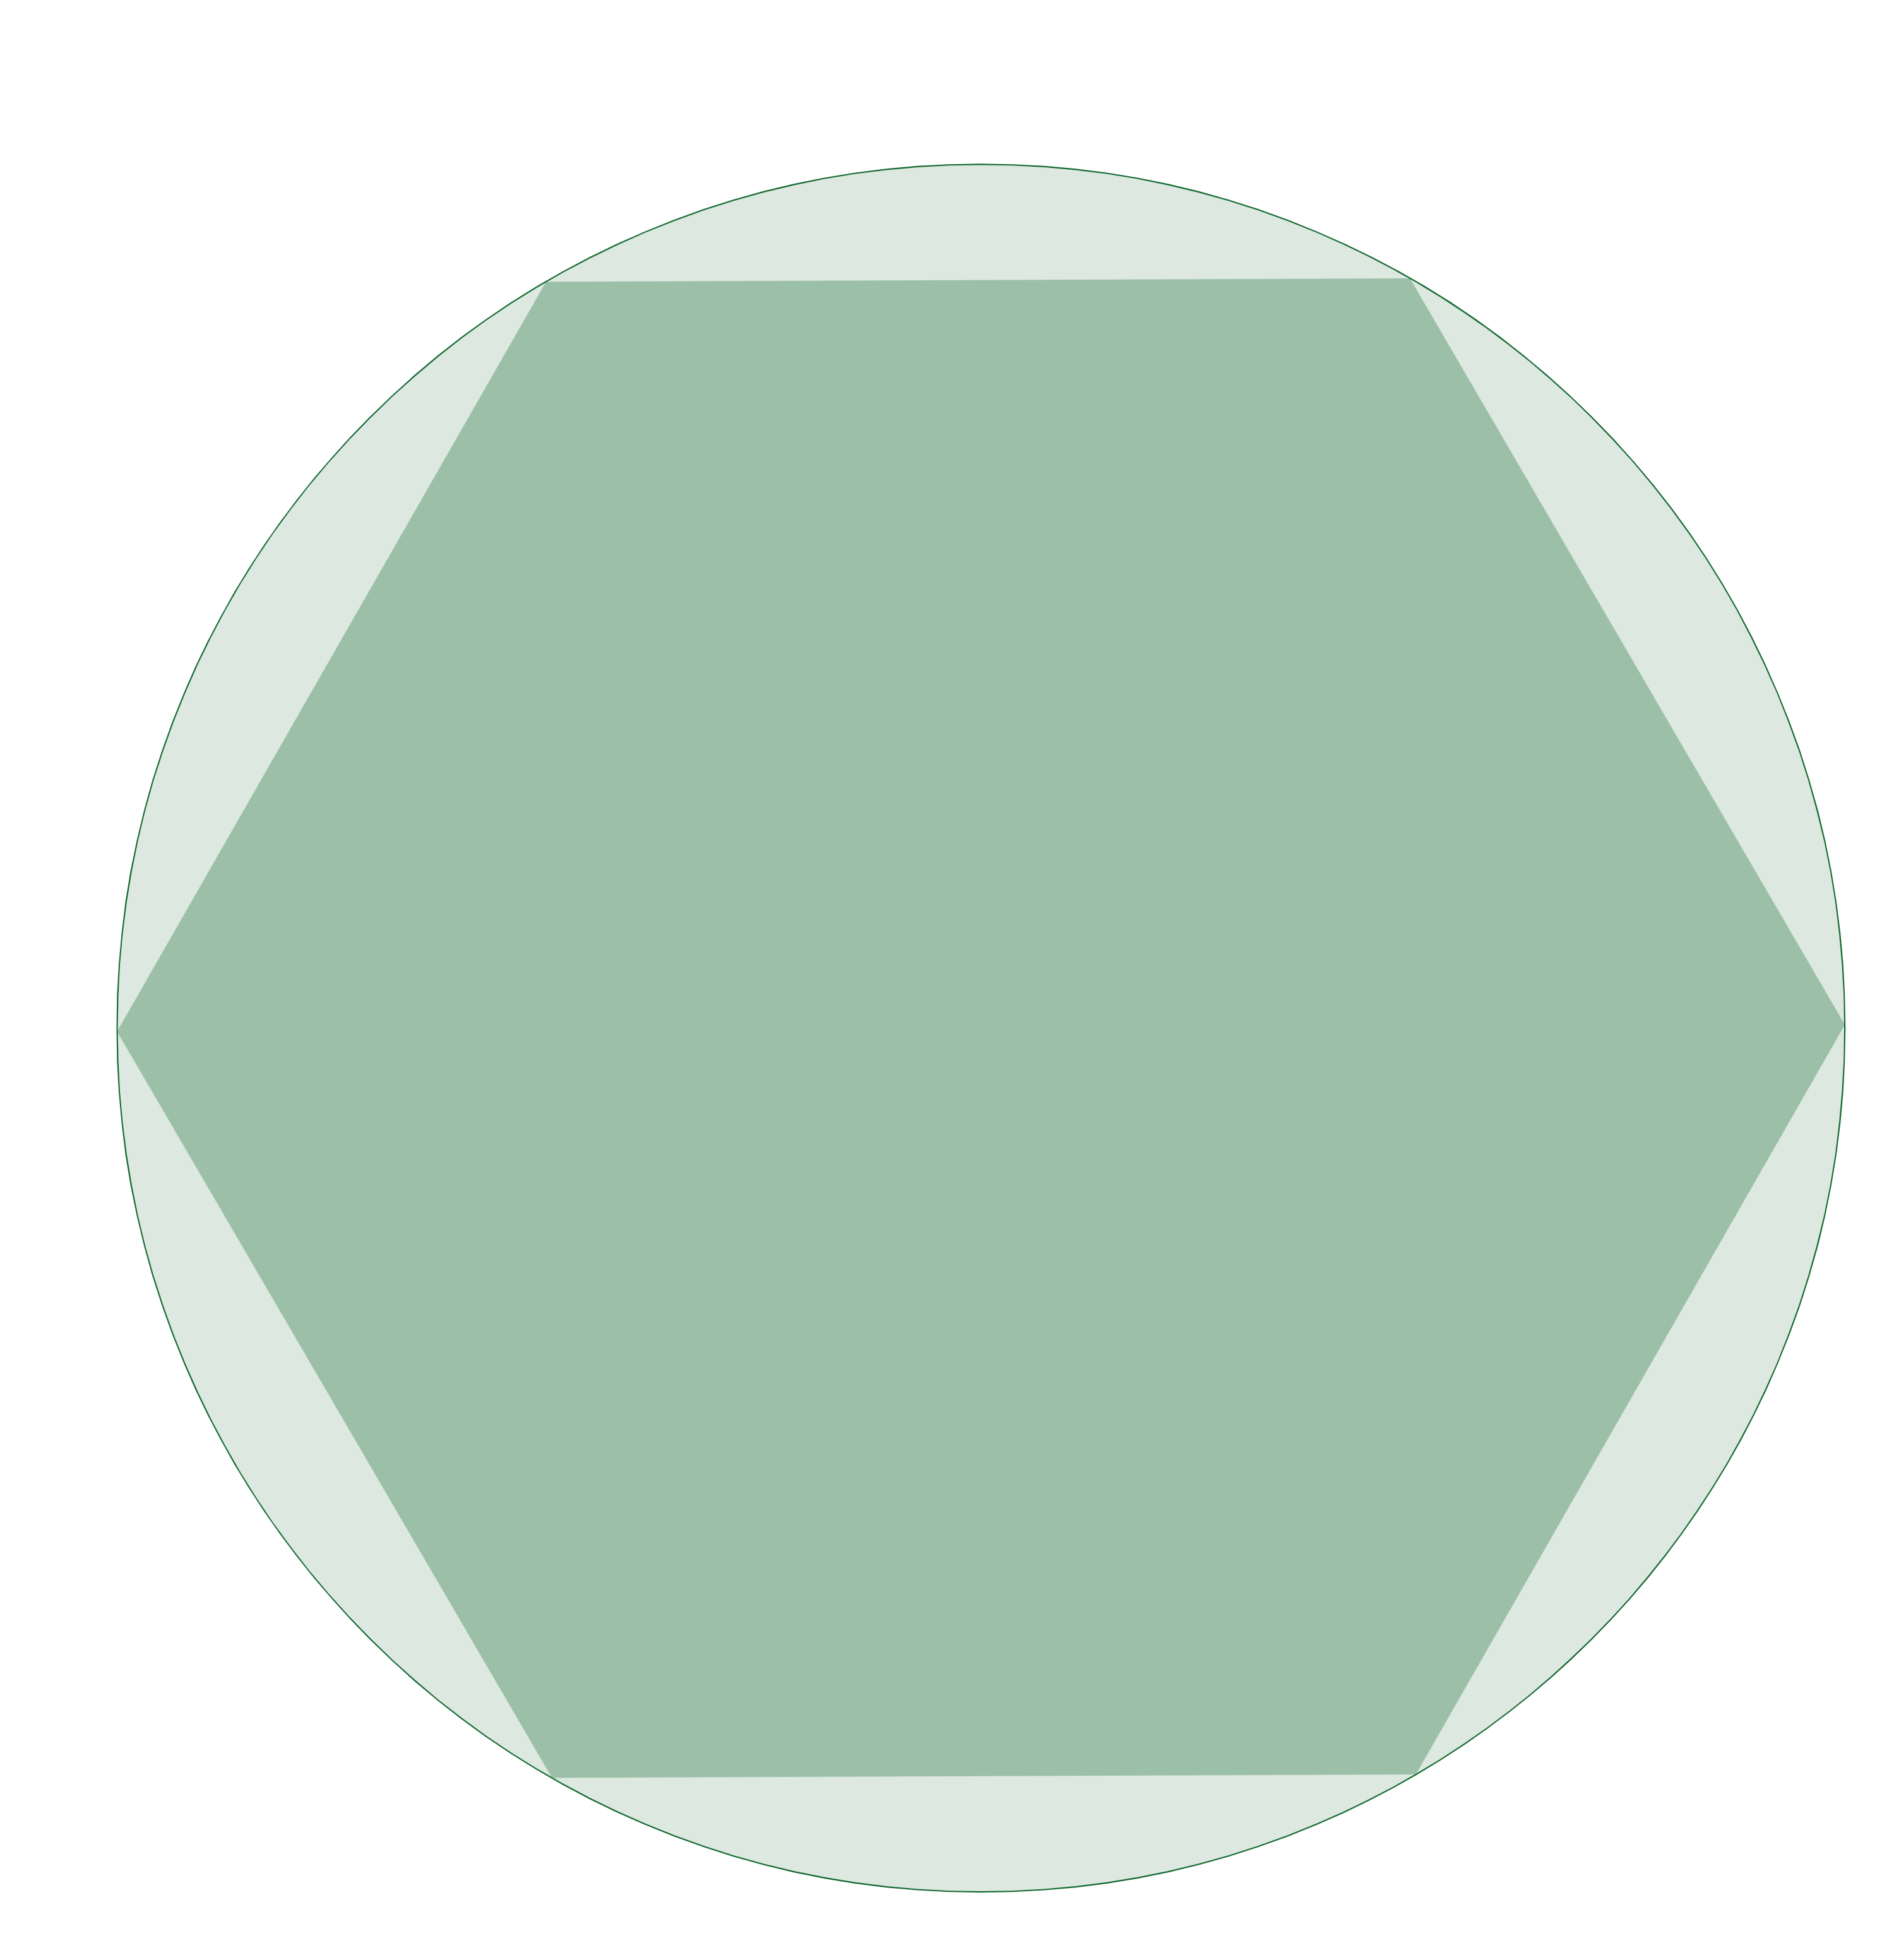
\includegraphics[scale=0.5]{img/fig1.png}
	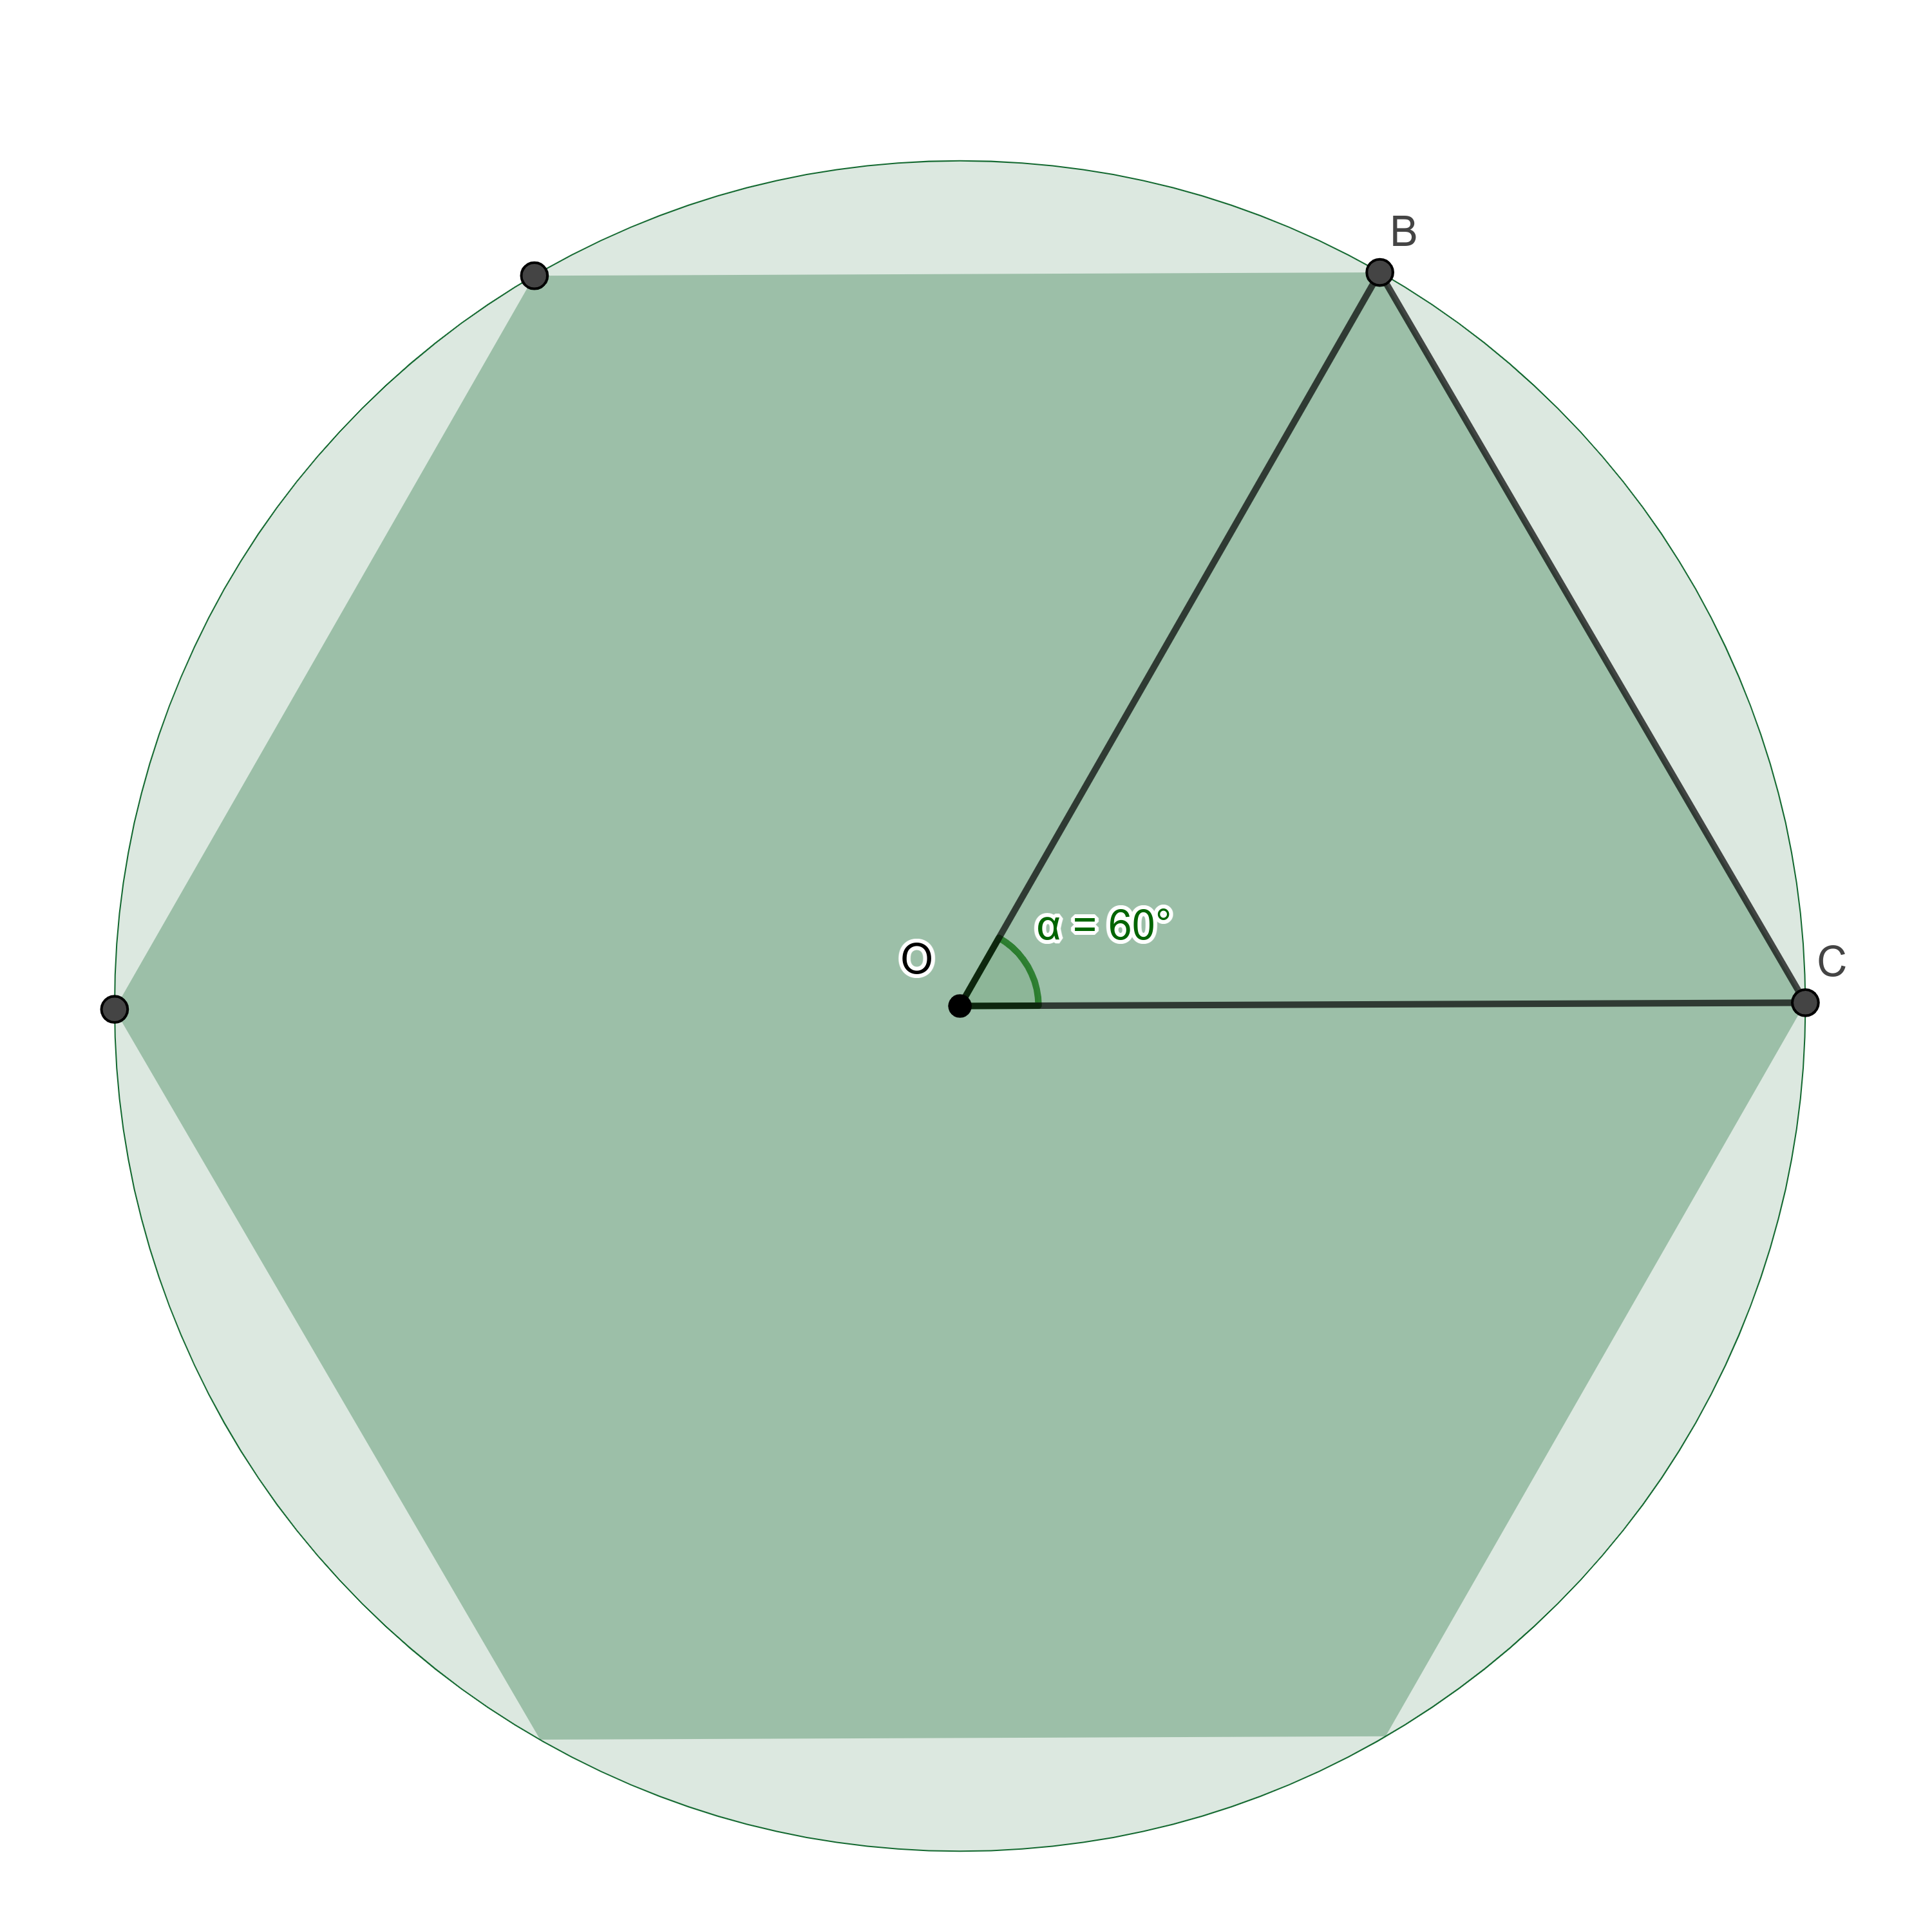
\includegraphics[scale=0.5]{img/fig2.png}
	\label{fig:1}
\end{figure}

Y a partir de el área de uno de los tríangulos isósceles que se forman, calcular el área del polígono. A medida que aumentamos el número de nodos del polígono, el área de este se aproxima cada vez más al área del círculo. Por lo que si llamamos $P_n$ a un polígono de $n$ lados inscrito en el círculo podemos decir que:
$$A_{\text{círculo}}=\lim_n A_{P_n} $$

Con una idea similar se comenzó a trabajar para calcular el área de cualquier figura plana, en especial del área bajo la curva de una función real. Pongamos como ejemplo la función $f(x)=x^2$ para $x>0$.
\begin{figure}[h!]
	\centering
	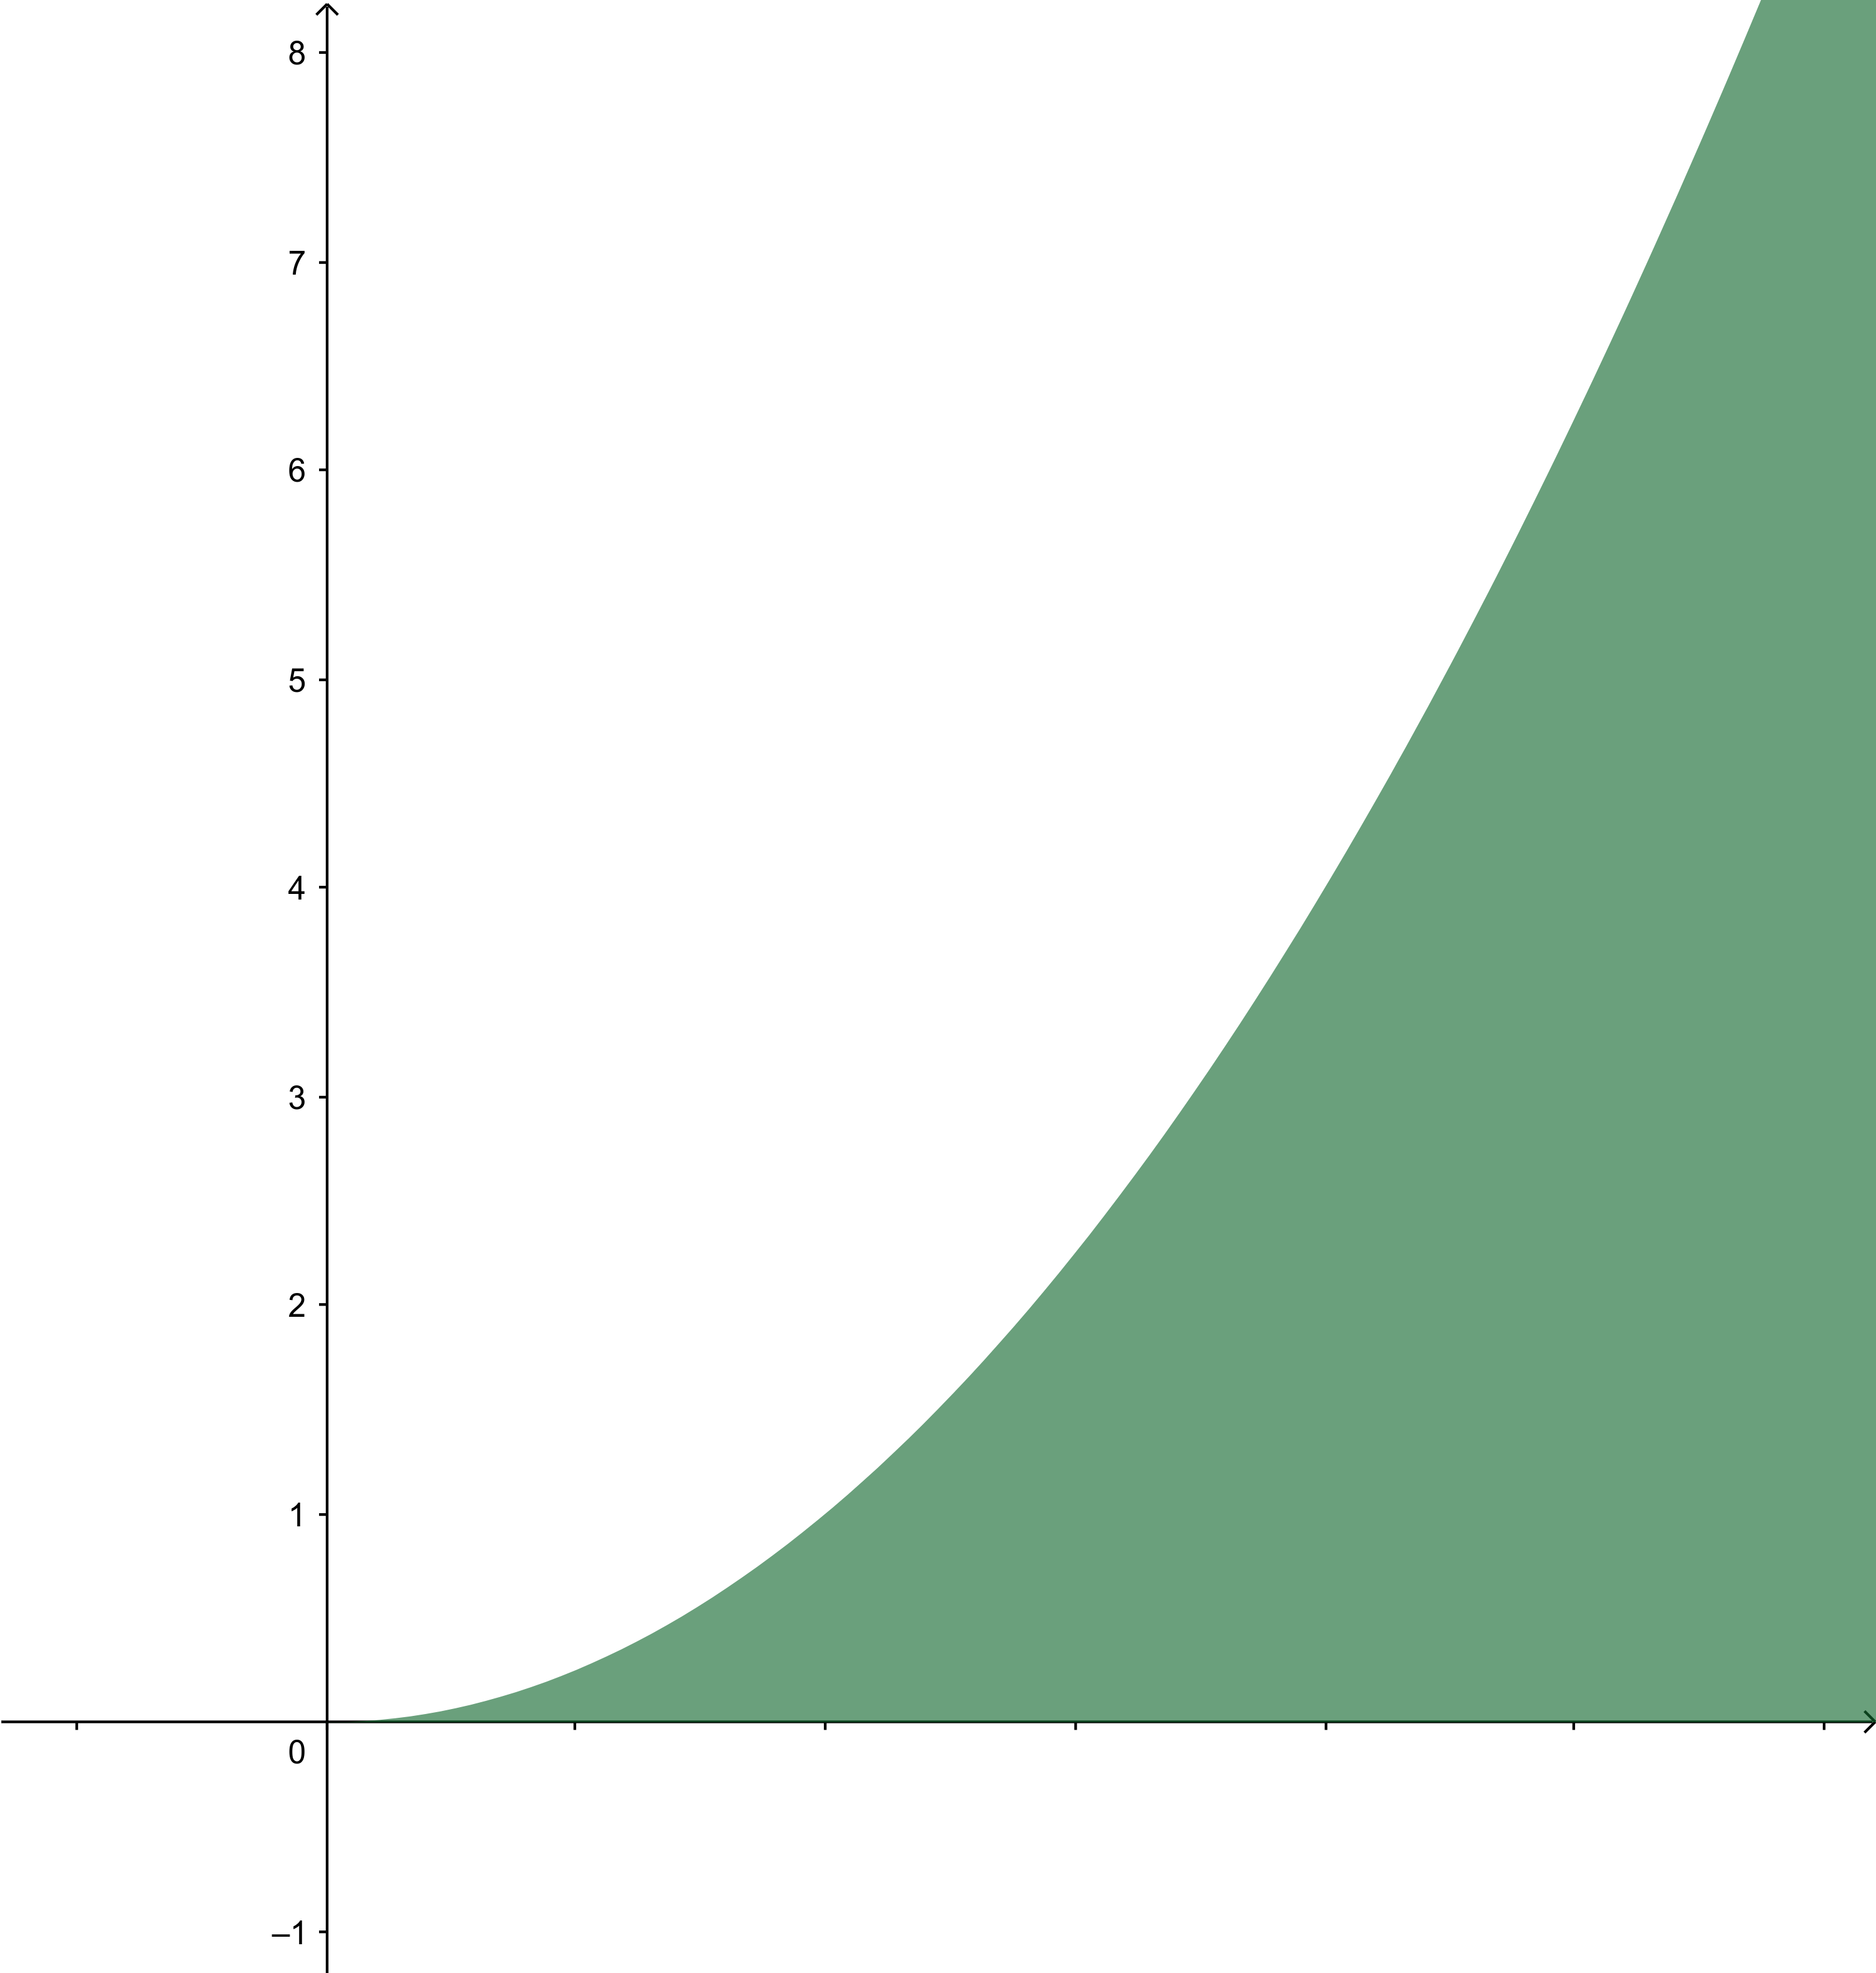
\includegraphics[scale=2]{img/fig3.png}
	\label{fig:2}
\end{figure}
\newpage
Para este caso se comienzan a hacer subdivisiones del intervalo, en este caso tomaremos una partición $\displaystyle P=\{x_i\}_0^{n}$ y formaremos rectángulos tanto superiores como inferiores a la curva:
\begin{figure}[h!]
	\centering
	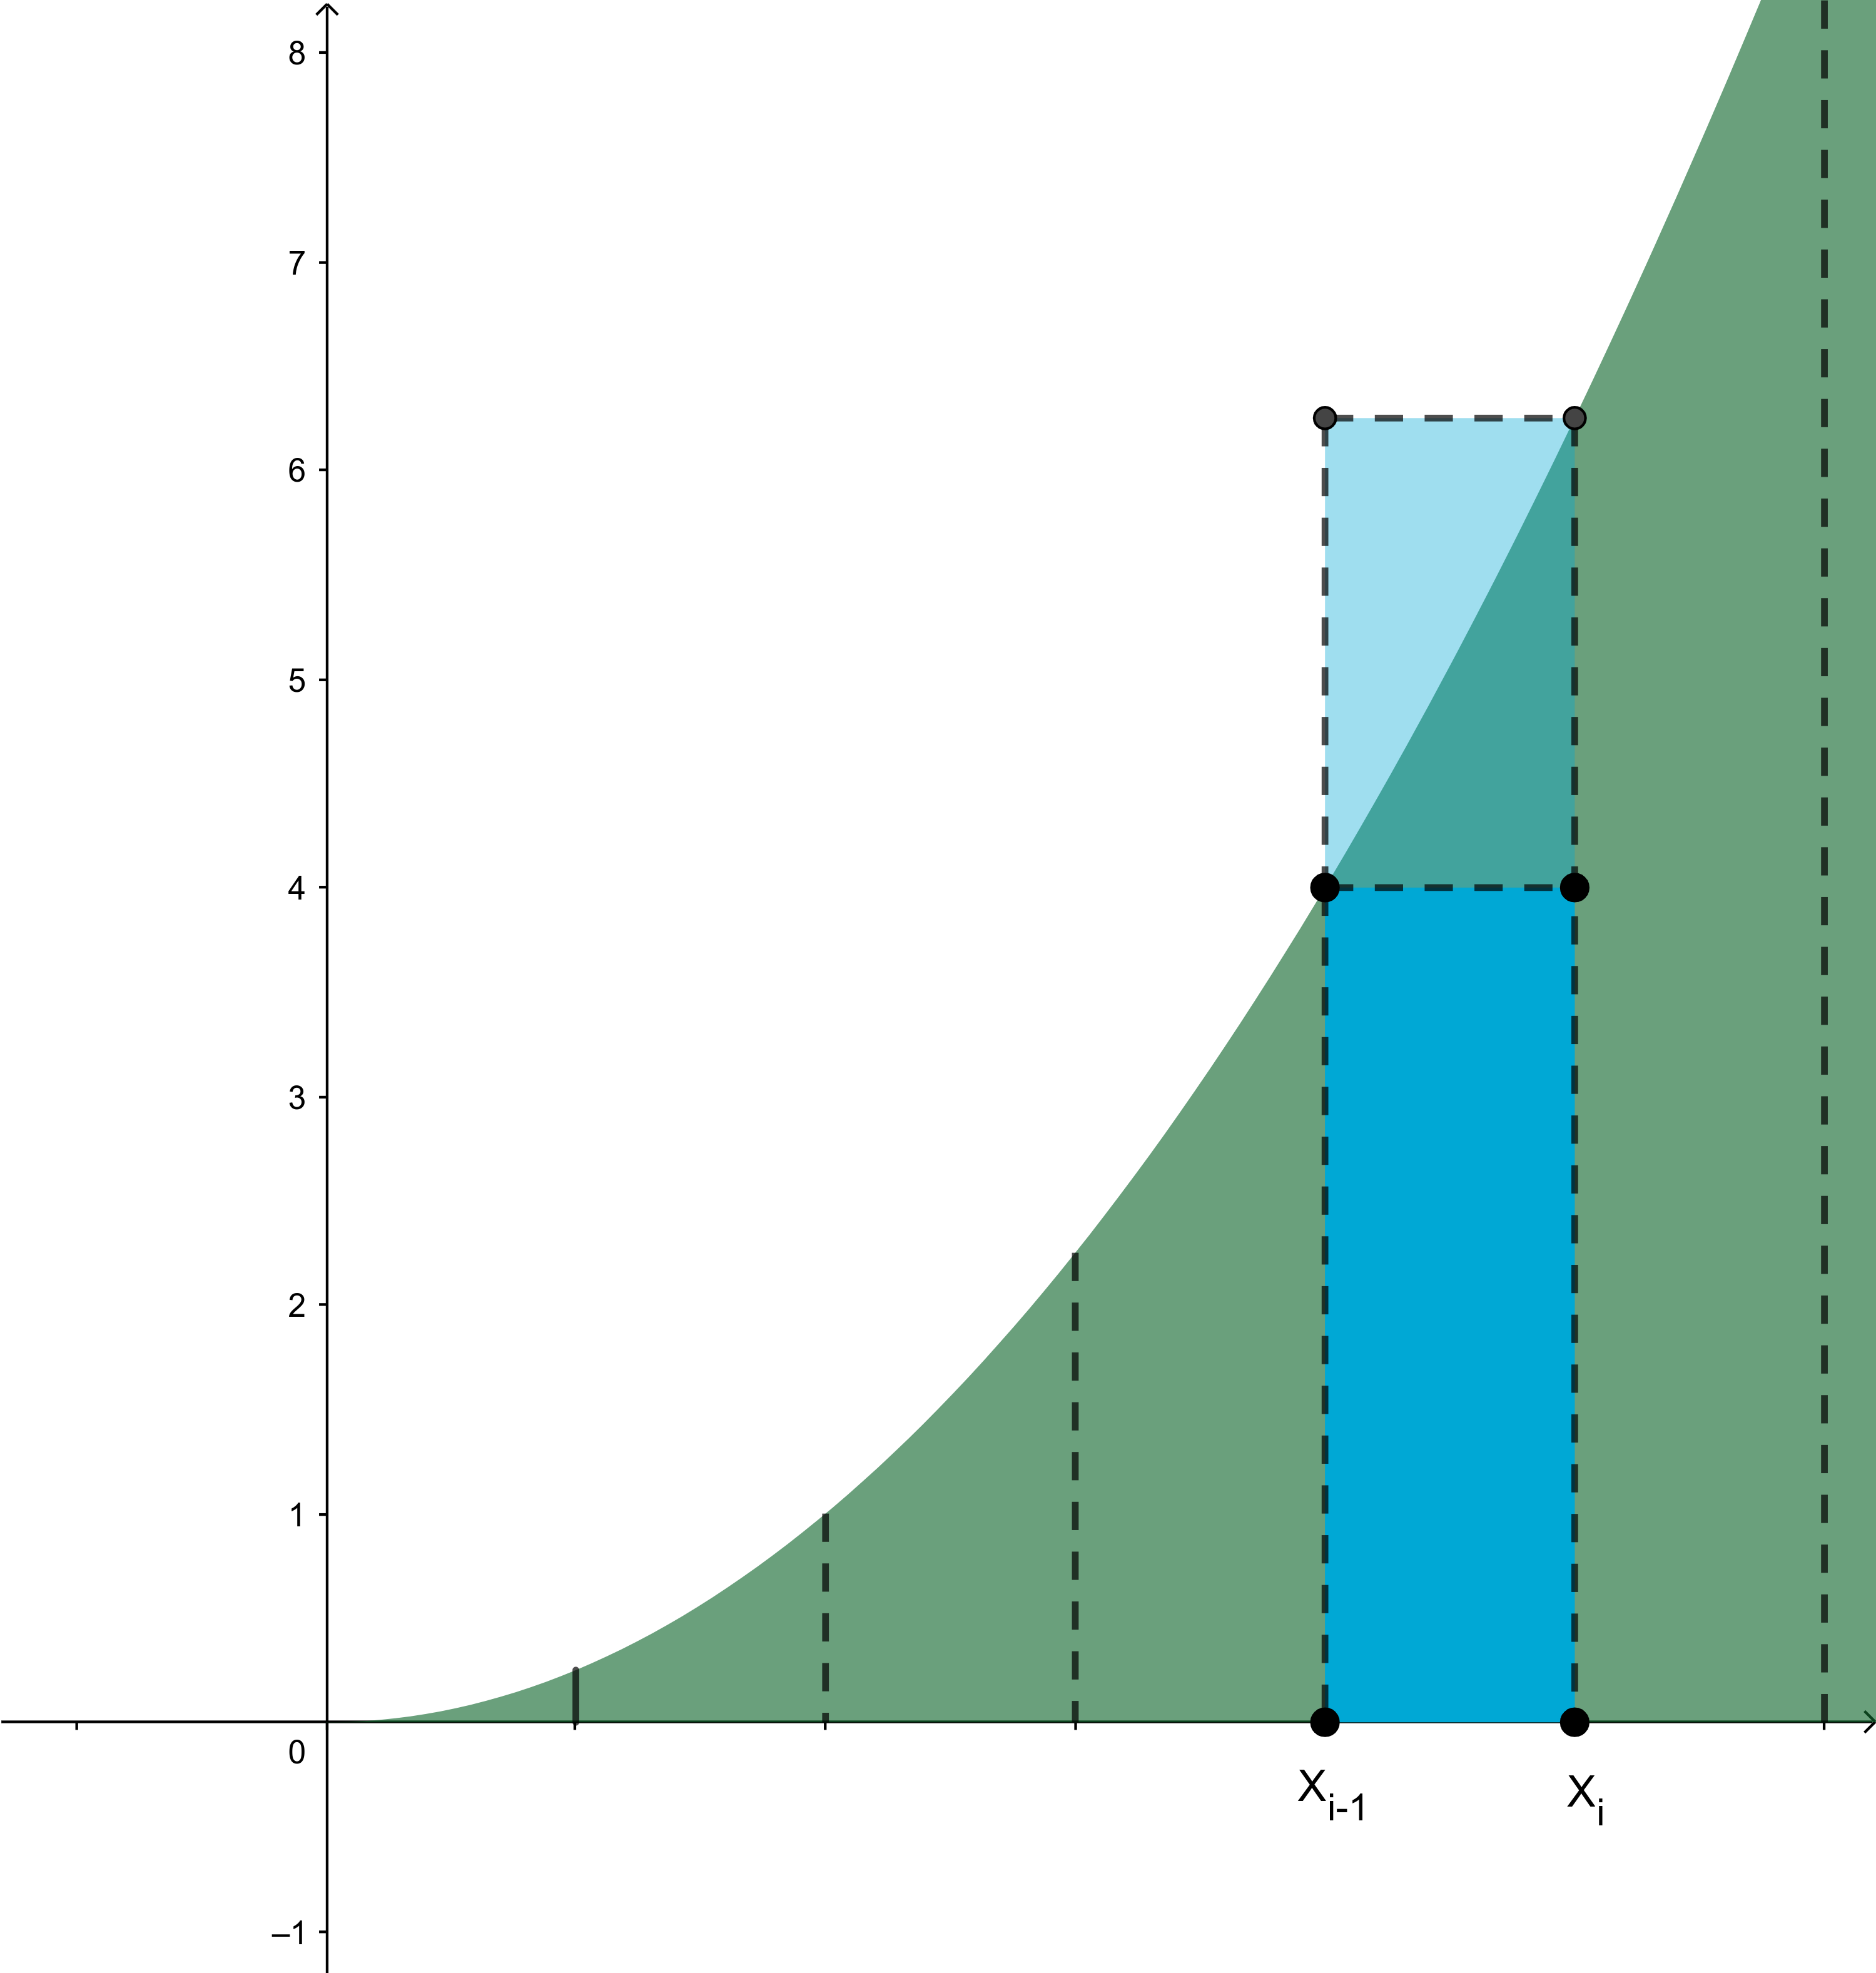
\includegraphics[scale=2]{img/fig5.png}
\end{figure}

A medida que aumentamos el tamaño de la partición los rectángulos superiores se acercan a los inferiores, por lo que podemos afirmar que el área de la región se encuentra comprendida entre la unión de las áreas de los rectángulos superiores y la unión de las áreas de los rectángulos inferiores, por lo que tendríamos un aproximado del área de interés.
\begin{center}
	{\color{uprgreen}--------------------------------------------------------------------------------------------------------------------------------------------}
\end{center}
Sea la función $f:\mathbb{R}\rightarrow\mathbb{R}$ y la partición $P=\{x_i\}_0^n$ equidistante de tamaño $\Delta x_i$, es decir $\Delta x_i=x_i-x_{i-1}$, podemos decir que el área de cada rectángulo formado superior tiene como expresión:
$$A_{\text{RS}}^i=f(x_i)(x_i-x_{i-1})$$
y para los rectángulos inferiores:
$$A_{\text{RS}}^i=f(x_{i-1})(x_i-x_{i-1})$$
y a partir de estos definir las conocidas como sumas de Darboux:
$$s_p=\sum_{i=0}^nm_i\Delta x_i$$
donde $m_i=\inf_{[x_{i-1},x_i]}f(x)$, y $s_p$ es la {suma inferior de Darboux}.\\ \\
Siguiendo la misma idea también podemos obtener las llamadas sumas superiores de Darboux de la siguiente manera:
$$S_p=\sum_{i=0}^nM_i\Delta x_i$$
donde $M_i=\sup_{[x_{x-1},x_i]}f(x)$.

Llamaremos integral de una función $f$, $I(f)=\int f(x)dx$ al área bajo la curva de la función $f$. Como veníamos anunciando desde la introducción $s_p\leq \text{área bajo la curva}\leq S_p$.

Definamos $\underline{I}$ como $\underline{I}=\sup_ps_p$ y $\overline{I}$ como $\overline{I}=\inf_pS_p$.
\\ \\
{\bf Definimos} como {\it norma de la partición $P$} $$\lambda(P)=\max_{0\leq i\leq n} \Delta x_i,\ \text{donde}\ \Delta x_i=x_i-x_{i-1}$$\\ \\
{\bf Teorema} $f$ es Darboux integrable $\Leftrightarrow \lim_{\lambda(P)\rightarrow 0}(S_p-s_p)=0$ y $\underline{I}=I=\overline{I}$.\\ \\
{\bf Teorema} Si la función f es continua, entonces las sumas de Darboux son sumas integrales.\\ \\ \\
Llamaremos suma {\it integral de Riemann} de $f$ respecto a la partición  $P$ a:
$$\sigma_f(P,\eta_i)=\sum_{i=1}^nf(\eta_i)\Delta x_i,\ \text{con}\ \eta\in[x_{i-1},x_i], (i=1,2,...,n)$$

Diremos que $f$ es integrable según Riemann en un compacto, si existe:
$$I=\lim_{\lambda(P)\rightarrow 0}\sigma_f(P,\eta_i)$$

$I$ la nombramos como {\it integral de $f$} y se denota:
$$I(f)=\int f(x)dx$$
en el caso restringir la integral a un intervalo $[a,b]$ se denotaría:
$$I=\int_a^bf(x)dx$$
$a$ y $b$ son llamados límites de integración.\\ \\

$$s_p\leq \sigma(P,\eta)\leq S_p,\ \forall P$$

De ahí que si una función $f$ es Riemann integrable entonces es Darboux integrable y viceversa.
\\ \\
{\bf Teorema:} Toda función continua en un intervalo $[a,b]$ es Riemann integrable en $[a,b]$.\\ \\
{\bf Colorario:} Si una función $f$ tiene sólo un número finito de discontinuidades (tipo salto o evitable) en $[a, b]$, entonces $f$ es Riemann-integrable en $[a, b]$.\\ \\
A partir de la definción se pueden obtener algunas propiedades fundamentales del cálculo integral.
\begin{enumerate}
	\item Sean $f$,$g\in R[a,b]$ y $\alpha,\beta\in\mathbb{R}\Rightarrow \alpha f+\beta g\in R[a,b]$ y se cumple que:
	$$\int_a^b(\alpha f+\beta g)(x)dx=\alpha\int_a^b f(x)dx+\beta\int_a^bg(x)dx$$
	\item Si $f\in R[a,b]$ y $[\alpha,\beta]\subset[a,b]\Rightarrow f\in R[\alpha,\beta]$
	\item Si $a<c<b$, $f\in R[a,c]$ y $f\in R[c,b]\Rightarrow f\in R[a,b]$ y se cumple:
	$$\int_a^b f(x)dx=\int_a^cf(x)dx+\int_c^bf(x)dx$$
	\item Si $\displaystyle f\in R[a,b],\ f(x)\geq 0, \forall x\in[a,b]\Rightarrow \int_a^bf(x)dx\geq0$
	\item Sean $\displaystyle f,g\in R[a,b],\ f(x)\leq g(x)\ \forall x\in[a,b]\Rightarrow \int_a^bf(x)dx\leq\int_a^bg(x)dx$
\end{enumerate}
A pesar de que la propia definición de la integral nos denota un método para su cálculo, este es demasiado complicado como para realizarlo en la mayoría de los casos. De ahí que se hayan obtenido herramientas para facilitar el cálculo integral. Veamos ahora algunos resultados de integrales inmediatas de las llamadas integrales indefinidas:
\begin{enumerate}
	\item $\displaystyle \int 0dx=c$, donde $c\in\mathbb{R}$
	\item Sea $a\in\mathbb{R}$ y $n\in\mathbb{Z}, n\neq-1\Rightarrow$ $\displaystyle \int ax^ndx=\dfrac{a}{n+1}x^{n+1}+c$, donde $c\in\mathbb{R}$
	\item $\displaystyle\int\dfrac{1}{x}dx=ln(x)+c$, donde $c\in\mathbb{R}$
	\item $\displaystyle\int e^x=e^x+c$, donde $c\in\mathbb{R}$
	\item Sea $\displaystyle a\in\mathbb{R}, a>0\Rightarrow \int a^xdx=\dfrac{a^x}{\ln a}+c$, donde $c\in\mathbb{R}$
	\item $\displaystyle \int\cos(x)dx=\sin(x)dx+c$, donde $c\in\mathbb{R}$
	\item $\displaystyle \int\sin xdx=-\cos xdx+c$, donde $c\in\mathbb{R}$
	\item $\displaystyle \int\dfrac{1}{\cos^2 x}dx=\tan x+c$, donde $c\in\mathbb{R}$
	\item $\displaystyle \int-\dfrac{1}{\sin^2 x}dx=\text{cot}\ x+c$, donde $c\in\mathbb{R}$
\end{enumerate}

{\bf Ejemplo:} Calcula las siguientes integrales indefinidas:
$$a) \displaystyle \int (3\sin(x)+x)dx$$
A partir de las propiedades vistas anterioremente podemos resolver esta integral de la siguiente manera:

\begin{align*}
	\int (3\sin(x)+x)dx&=\int 3\sin(x)dx+\int xdx=3\int\sin(x)dx+\int xdx\\
	&=-3\cos(x)+c_1+\dfrac{x^2}{2}+c_2\\
	&=-3\cos(x)+\dfrac{x^2}{2}+C
\end{align*}
$$b) \displaystyle \int \dfrac{\sin(2x)}{\cos(x)}dx$$
Sabemos de trigonometría que:
$$\sin(2x)=2\sin(x)\cos(x)$$
luego:
\begin{align*}
	\int \dfrac{\sin(2x)}{\cos(x)}dx&=\int\dfrac{2\sin(x)\cos(x)}{\cos(x)}dx\\
	&=\int2\sin(x)dx\\
	&=2\int\sin(x)dx\\
	&=-2\cos(x)+c
\end{align*}
\begin{center}
	{\color{uprgreen}--------------------------------------------------------------------------------------------------------------------------------------------}
\end{center}

{\bf Ejercicios de estudio independiente}\\ \\
Calcule las siguientes integrales:
\begin{enumerate}
	\item[]
	\begin{enumerate}
		\item $\displaystyle \int\dfrac{2}{x^3}dx$
		\item $\displaystyle \int\sqrt{1-\sin^2(x)}dx$
		\item $\displaystyle \int (x^4+3x^2+5)dx$
		\item $\displaystyle \int \left(e^x+\dfrac{1}{x}\right)dx$
	\end{enumerate}
\end{enumerate}

En la próxima clase abordaremos las integrales indefinidas inmediatas para funciones compuestas, las integrales definidas y principales métodos para el cálculo de integrales.
\end{document}
